\documentclass[10pt]{article}
\usepackage{listings}
\usepackage{float}
\usepackage{soul}
%\usepackage{svg}
\usepackage{algorithm}
\usepackage{algorithmic}
%\usepackage[]{algorithm2e}
\usepackage[superscript,biblabel]{cite}
\usepackage{graphicx}
\usepackage{subcaption}
\usepackage{fancyhdr}
\pagestyle{fancy}
%\lhead{CS7642 Reinforcement Learning 2018 Spring}
%\chead{ID: rchen350}
%\rhead{Assignment 3: Unsupervised Learning}
\fancyhead{} % clear all header fields
\fancyhead[L]{\fontsize{10}{12} \selectfont CS7641 Reinforcement Learning \\ 2018 Summer}
\fancyhead[C]{\fontsize{10}{12} \selectfont ID: rchen350 \\}
\fancyhead[R]{\fontsize{10}{12} \selectfont Project 3: RoboCup \\ \burl{https://github.gatech.edu/rchen350/cs7642summer2018p3}}

\lfoot{}
\cfoot{\thepage}
\rfoot{}
\renewcommand{\headrulewidth}{0.4pt}
\renewcommand{\headwidth}{\textwidth}
\renewcommand{\footrulewidth}{0pt}
%\usepackage{nips_2017}
\usepackage[utf8]{inputenc} % allow utf-8 input
\usepackage[T1]{fontenc}    % use 8-bit T1 fonts
\usepackage{hyperref}       % hyperlinks
\usepackage{url}            % simple URL typesetting
\usepackage{booktabs}       % professional-quality tables
\usepackage{amsfonts}       % blackboard math symbols
\usepackage{nicefrac}       % compact symbols for 1/2, etc.
\usepackage{microtype}      % microtypography
\usepackage{amsmath}
\DeclareMathOperator*{\argmax}{argmax} % thin space, limits underneath in displays
\DeclareMathOperator*{\argmin}{argmin} % thin space, limits underneath in displays
\DeclareMathOperator{\sgn}{sgn}
%\DeclareMathOperator*{\max}{max} % thin space, limits underneath in displays
%\DeclareMathOperator*{\min}{min} % thin space, limits underneath in displays
\usepackage{amssymb}
\usepackage{hyperref}
\usepackage{breakurl}
\usepackage[
			headheight=48pt, % height for the header block
			]{geometry}
\geometry{letterpaper, portrait, margin=1in}
\setlength\parindent{24pt}

\author{Ran Chen \\ email: ranchen@gatech.edu\vspace{-2ex}}
\title{\vspace{-1.8cm}Project 3: RoboCup}
\date{}
\begin{document}
\maketitle
\thispagestyle{fancy}


\section{Game: Soccer} \label{game}

\ul{\textbf{Game}} The soccer game is grid game of 2 rows and 8 columns, with two players A and B, as shown in \textbf{Fig} \ref{fig:soccer}. The rules are determined according to the published description of the game, as well as some reasonable assumption, since a detailed list of rules is hardly presented in full in those publications. The rules are:\par


\begin{enumerate}
  \item The game is always initiated or reset to state s, as shown in \textbf{Fig} \ref{fig:soccer}, in which B holds the ball, occupying position $[0,1]$ and A occupies position $[0,2]$.
  \item Each player has two possible actions [stick, N, S, E, W], and the action vector is represented in that order, e.g. $[0.3,0,0.7,0,0]$ means moving South with 0.7 chance and stick with 0.3 chance.
  \item At each step of the game, A and B determines their moves simultaneously, but the execution of those two moves are always in random order.
  \item When a player with the ball is trying to move into the position already occupied by the other player, then the ball changes possession, and neither player changes position.
  \item When it ball is in a player's goal, then that player scores $100$, its opponent scores $-100$, and game ends, no matter who has the ball at the time.
  \item At a particular step of the game, game ending is only checked after the moves of both players are executed, i.e. even if the intermediate state of the game after the first move is executed includes the ball in the goal, the game does not end until the criteria is met after the second move is executed.
\end{enumerate}


%%%%%%%%%%%%%%%%%%%figure here v
\begin{figure}[h!]
  \centering
  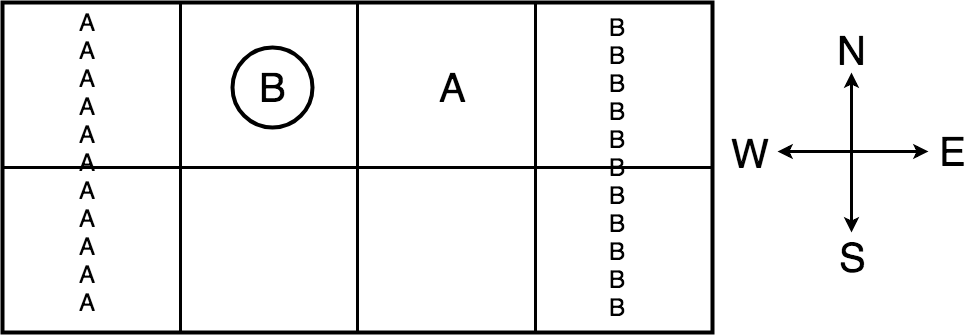
\includegraphics[width=0.65\linewidth]{diagram/soccer.png}
    \caption{An illustration of the soccer grid game environment. This illustration is showing the initial state of the game, state s. The circle on player B indicates B is in possession of the ball. 4 directions of movement are demonstrated on the right. The lines of A and B indicates the position of goals of respective player.}
  \label{fig:soccer}
\end{figure}
%%%%%%%%%%%%%%%%%%% figure here ^

\bigbreak
\noindent
\ul{\textbf{Approach}} Different variants of multiagent Q-learning algorithms will be tested with soccer environment. The generic algorithm\cite{GreenwaldCorrelatedQLearning2003} is shown in \textbf{Algorithm} \ref{alg:QL}. Note: here the term "off-policy" refers to Sutton's definition, more clarification presented \textbf{Section} \ref{clarification}.

\begin{algorithm}
\caption{Off-policy multiagent Q-Learning}\label{alg:QL}
\begin{algorithmic}
\STATE input: $f$ - strategy selection function; $\gamma$ - discount; $\alpha$ - learning rate; $D$ - decay schedule; $T$ - total training steps
\STATE output: action-value function $Q_i^*$
\STATE initialize $s$ and $Q_1,...Q_n$
\FOR{$t\in \{1,...,T\}$}
\STATE choose and execute actions $a_1,...,a_n$ at state $s$
\STATE observe rewards $R_1,...R_n$ and the next state $s'$
\FOR{$i\in \{1,...,n\}$}
\STATE $V(s')\leftarrow f_i(Q_1(s'),...,Q_n(s'))$
\STATE $Q_i(s,a_1,...,a_n)\leftarrow(1-\alpha)Q_i(s,a_1,...,a_n)+\alpha[(1-\gamma)R_i+\gamma V_i(s')]$
\ENDFOR
\STATE $s\leftarrow s'$
\STATE $\alpha\leftarrow D(\alpha)$
\ENDFOR
\end{algorithmic}
\end{algorithm}

\section{Clarifications: difficulties} \label{clarification}
Most of the difficulties I encountered in Project 3 were related to ambiguities in the descriptions of various learning algorithms and the game environment. After careful reading a few other related literature and consideration, the environment is re-defined in \textbf{Section} \ref{game}. A few additional clarifications regarding the algorithms need to be made before I can proceed.\par
\bigbreak
\noindent
\ul{\textbf{On/off-policy}} In Table 1 in Greenwald's technical report "Correlated Q-Learning", published in 2005\cite{GreenwaldCorrelatedQLearning2005}, on/off-policy seem to only affect how actions are chosen, not how state value $V(s')$ is evaluated. This means even for on-policy Q-learning, state value $V(s')$ is still evaluated using greedy policy $\pi_{s'}$ calculated from $Q(s')$. Such notion of on/off-policy is inconsistent with Sutton's definition\cite{SuttonReinforcementLearningIntroduction1998}. Here a distinction is made, since such notions are important for understanding how each variant of the algorithm performs in experiments.\par
\bigbreak
\noindent
First, define:
\begin{itemize}
   \item $\pi(s)$ as strategy calculated from $Q(s)$ (either mixed strategy obtained from linear programming or pure strategy using $\argmax$)
   \item $P\{\epsilon, \pi(s)\}$ as a $\epsilon$-greedy policy where random action is chosen with probability $\epsilon$, otherwise follow $\pi(s)$. In particular $P\{\epsilon\rightarrow 0.001, \pi(s)\}$ means $\epsilon$-greedy with $\epsilon$ decaying to 0.001, and $P\{\epsilon=1, \pi(s)\}$ means complete random action
\end{itemize}

 
\noindent
According to Sutton's definition\cite{SuttonReinforcementLearningIntroduction1998},  on/off policy affects how $V(s')$ is evaluated, not how action is chosen, then
\begin{itemize}
   \item On-policy: evaluate $V(s')$ using $P\{\epsilon, \pi(s')\}$, choose action using $P\{\epsilon, \pi(s')\}$
  \item Off-policy: evaluate $V(s')$ using $\pi(s')$, choose action using $P\{\epsilon, \pi(s')\}$
\end{itemize}

\noindent
According to Greenwald's definition\cite{GreenwaldCorrelatedQLearning2005}, on/off policy affects how action is chosen, not $V(s')$ evaluation,
\begin{itemize}
  \item On-policy: evaluate $V(s')$ using $\pi(s')$, choose action using $P\{\epsilon\rightarrow 0.001, \pi(s')\}$
  \item Off-policy: evaluate $V(s')$ using $\pi(s')$, choose action using $P\{\epsilon=1, \pi(s')\}$
\end{itemize}
 

In this report, we follow Sutton's definition, Greenwald's both on- and off-policy are actually off-policy, just with different exploration strategy, $\epsilon\rightarrow 0.001$ \textit{vs}. $\epsilon=1$.
\bigbreak
\noindent
\ul{\textbf{Strategy selection function}} The strategy selection function $f$ from the algorithm shown above is the determining factor for each variant of multiagent Q-Learning. In regular Q-Learning, the agents are unaware of the existence of other players, but can observe the state of the game in full, so every agent just learn its own Q function, thus an agent maximizes values of its own actions $\max Q(s,a)$. In friend-Q\cite{LittmanFriendorFoeQlearningGeneralSum2001}, a particular agent $A$ maximizes its own payoff at each state, and assumes the other players will coordinate their choices to let agent $A$ receive the maximum payoff, thus an agent evaluate state value using $\max Q(s,\vec{a})$. Foe-Q\cite{LittmanFriendorFoeQlearningGeneralSum2001} incorporate mixed strategies for individual actions at Nash equilibrium using maximin algorithm. Correlated-Q (CE-Q)\cite{GreenwaldCorrelatedQLearning2003} employs mixed strategies for joint actions at correlated equilibrium.
\bigbreak
\noindent
\ul{\textbf{Iteration}} Greenwald's 2003 paper\cite{GreenwaldCorrelatedQLearning2003} is quite ambiguous on how a "iteration" is defined in their plots Q value differences during training. After carefully reading the paper, and experimenting with different assumptions, it is determined that one iteration means one step in the game, however the $Q(state=s,action=S)$ is not plotted at all steps, just the steps where it is updated. Later it is further discovered even that would make the figures too dense, only plotting the values when it is updated, and at a interval would generate figures as sparse as in the paper.
\bigbreak
\noindent
\ul{\textbf{Identical plots}} Greenwald's 2003 paper\cite{GreenwaldCorrelatedQLearning2003} presented identical plots for foe-Q and ce-Q, and explained both algorithm seeks Nash equilibrium for a zero-sum game. This is true, however, in both algorithms, actions are chosen randomly with $\epsilon$ probability (either $\epsilon=1$ or $\epsilon:1\rightarrow0.001$, see explanation above), thus it is impossible to generate identical plots for two algorithms that both involve significant amount of stochasticity, unless a fixed random number seed is defined. In my experiments, I did not set random seed, since that would not be a good experiment design for random processes, and my plots for foe-Q and CE-Q are not identical but similar as a result.




\section{Experiments and Results} \label{experiments}
Experiments presented in Fig 3 in Greenwald paper\cite{GreenwaldCorrelatedQLearning2003} were replicated. Q, friend-Q, foe-Q, and CE-Q were tested on soccer environment using different parameters, and their results and performances were compared. The Q values at a particular state action pair for player A, $Q(state=s, action=S)$ is recorded during training iterations.
\par

%%%%%%%%%%%%%%%%%%%figure here v

%%%%%%%%%%%%%%%%%%% figure here ^


\subsection{Q-Learning} \label{Q}
First, regular Q-Learning is tested with off-policy $\epsilon$-greedy with $\epsilon:1\rightarrow 0.001$ (off-policy by Sutton's definition\cite{SuttonReinforcementLearningIntroduction1998}, or on-policy by Greenwald's\cite{GreenwaldCorrelatedQLearning2005}). The other training parameter includes: learning rate $\alpha\rightarrow 0.001$, discount $\gamma=0.9$. In Q-Learning, the two agents are not aware of the actions taken by their opponents, only themselves, however they can observe the state of the game in full, i.e. player A can observe position of B, as well as possession of the ball, and vice versa. Here, since a player is only aware of its own action, it simply choose the action with the largest Q value at a particular state to evaluate the utility of that state.\par

As shown in \textbf{Fig} \ref{fig:Q09_y_cut} and \ref{fig:Q015_y_cut}, Q-Learning does not converge after $1\times10^6$ iterations. The reason for decreasing Q-value difference is the same as what is stated in the paper: decreasing learning rate $\alpha$. \textbf{Fig} \ref{fig:Q09_y_uncut} and \ref{fig:Q015_y_uncut} are a zoomed out view to show the entire range of Q-value differences, larger initial value of $\alpha$ produced higher Q value differences in early stages of the learning, but does not help with convergence. Note that with $\alpha$ initialized at both 0.9 and 0.15, the learning curve, with y-axis capped at 0.5, look \ul{very similar to the one presented in the paper}\cite{GreenwaldCorrelatedQLearning2003}. And the only difference of using different $\alpha$ seems to be the scale of Q-value difference, both converges within $1\times10^6$ steps and to the same policy, this behavior is also observed in cases of foe-Q and CE-Q, however in friend-Q, on optimal $\alpha$ is required to converge as fast as possible.\par



%%%%%%%%%%%%%%%%%%%figure here v
\begin{figure}[H]
  \centering
  \begin{subfigure}[b]{0.245\linewidth}
  \centering
  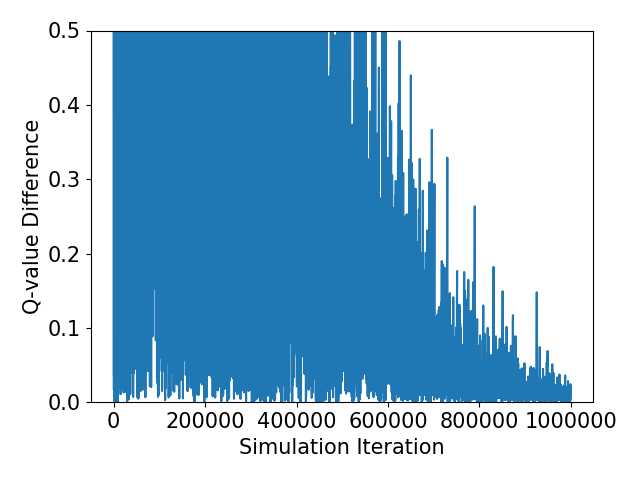
\includegraphics[width=\linewidth]{../figs/Q_offpolicy_09_1_1000000_replot.png}
      \caption{$\alpha:0.9\rightarrow0.001$}
  \label{fig:Q09_y_cut}
  \end{subfigure}
  \begin{subfigure}[b]{0.245\linewidth}
  \centering
  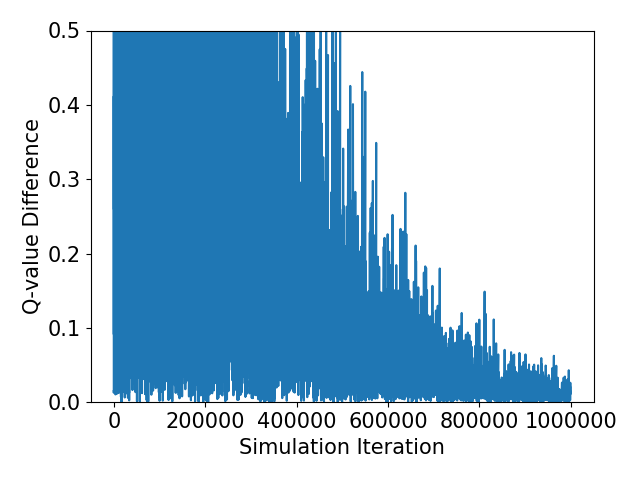
\includegraphics[width=\linewidth]{../figs/Q_offpolicy_015_0001_1_0001_1000000.png}
      \caption{$\alpha:0.15\rightarrow0.001$}
  \label{fig:Q015_y_cut}
  \end{subfigure}
  \begin{subfigure}[b]{0.245\linewidth}
  \centering
  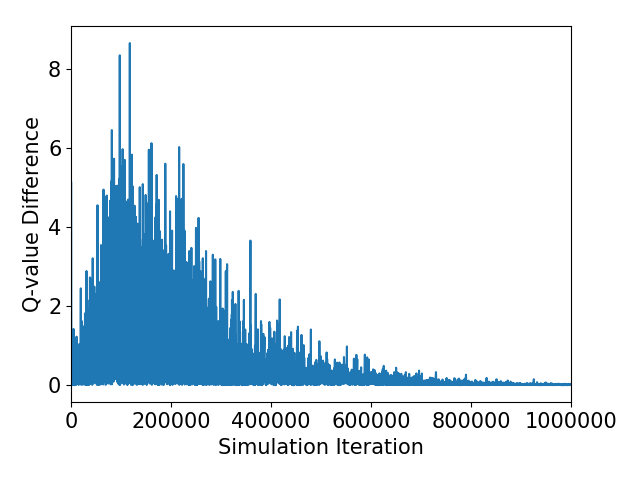
\includegraphics[width=\linewidth]{../figs/Q_offpolicy_09_1_1000000_uncut.png}
      \caption{$\alpha:0.9\rightarrow0.001$}
  \label{fig:Q09_y_uncut}
  \end{subfigure}
  \begin{subfigure}[b]{0.245\linewidth}
  \centering
  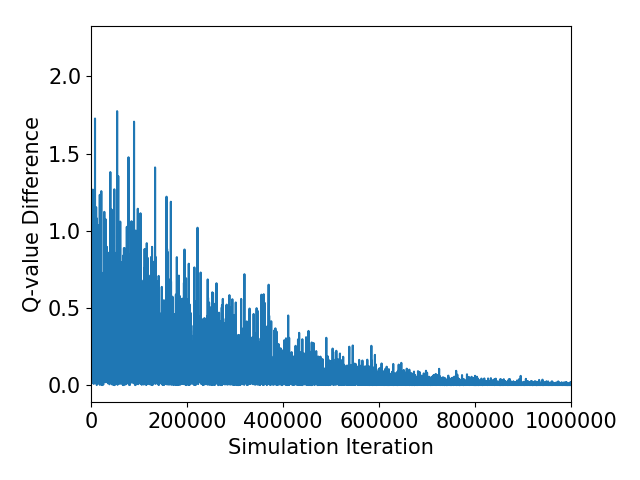
\includegraphics[width=\linewidth]{../figs/Q_offpolicy_015_0001_1_1_1000000_uncut.png}
      \caption{$\alpha:0.15\rightarrow0.001$}
  \label{fig:Q015_y_uncut}
  \end{subfigure}
  \caption{Q-value differences during training, at different initial values of $\alpha$, for Q-Learning, zoomed-in (a and b), and zoomed-out (c and d). \ul{Here (a) corresponds to Fig 3(d) in Greenwald2003 paper.}\cite{GreenwaldCorrelatedQLearning2003}}
  \label{fig:QL}
\end{figure}

%%%%%%%%%%%%%%%%%%% figure here ^



\subsection{Friend-Q} \label{friendQ}
In friend-Q\cite{LittmanFriendorFoeQlearningGeneralSum2001, GreenwaldCorrelatedQLearning2003, GreenwaldCorrelatedQLearning2005}, a player, A, is aware of actions of all players, as well as the full state of game, however in evaluating the utility of a particular state, it chooses the joint action with the highest Q value, and assumes its opponent will cooperate and let it choose that joint action. The opponent behaves the same, assuming A will cooperate with it.\par

Here, friend-Q is tested with $\alpha:0.2\rightarrow0.001$, \textbf{Fig} \ref{fig:friendQ_2Q_1} and \ref{fig:friendQ_2Q_0001} show the result from friend-Q learning two Q tables for both players, using off-policy learning with $\epsilon=1$ and $\epsilon:1\rightarrow0.001$ respectively (or off- and on-policy respectively defined by Greenwald\cite{GreenwaldCorrelatedQLearning2005}, detailed explanation see \textbf{Section} \ref{clarification}). \ul{Similar to the figure presented in the paper}\cite{GreenwaldCorrelatedQLearning2003}, friend-Q converges very fast, with \ul{$\pi_A(s)$ converging to a particular action randomly, and $\pi_B(s)=E$}.\par
Results described above were obtained by learning Q tables for A and B separately. Learning only one Q table is also feasible, by assuming the payoff matrix at any particular state is always opposite for the two players. The result obtained from learning a single Q table is shown in \textbf{Fig} \ref{fig:friendQ_1Q_1} and \ref{fig:friendQ_1Q_0001}, \ul{also comparable to the results shown in the paper}\cite{GreenwaldCorrelatedQLearning2003}. Same as the paper, \ul{$\pi_A(s)$ converges to a particular action randomly, and $\pi_B(s)=E$}.

%%%%%%%%%%%%%%%%%%%figure here v
\begin{figure}[H]
  \centering
  \begin{subfigure}[b]{0.245\linewidth}
  \centering
  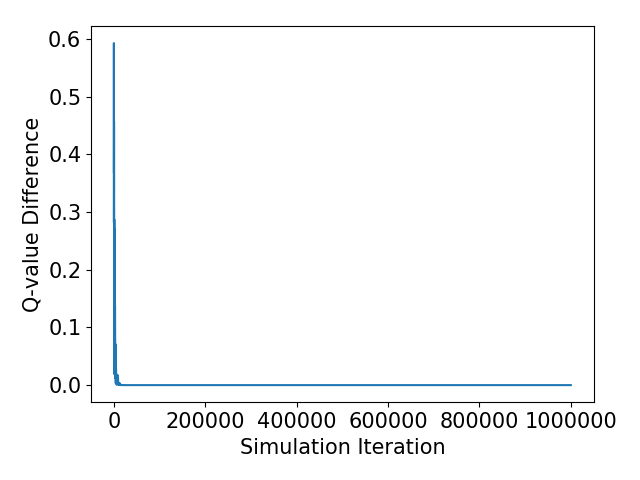
\includegraphics[width=\linewidth]{../figs/Qdifference_27_uncut.png}
      \caption{2 Q tables ($\epsilon=1$)}
  \label{fig:friendQ_2Q_1}
  \end{subfigure}
  \begin{subfigure}[b]{0.245\linewidth}
  \centering
  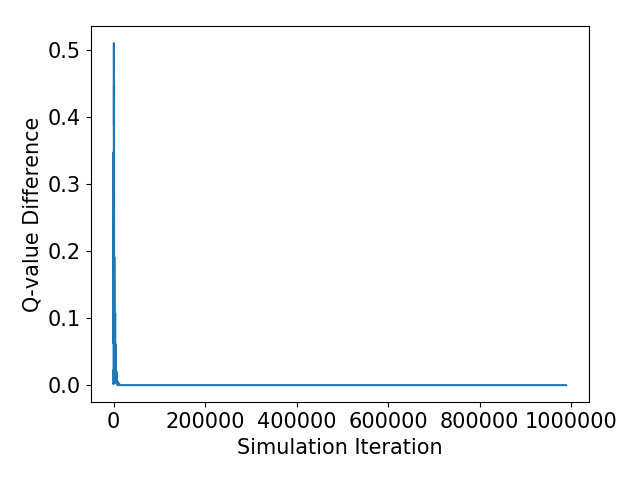
\includegraphics[width=\linewidth]{../figs/Qdifference_26_uncut.png}
      \caption{2 Q tables ($\epsilon:1\rightarrow0.001$)}
  \label{fig:friendQ_2Q_0001}
  \end{subfigure}
  \begin{subfigure}[b]{0.245\linewidth}
  \centering
  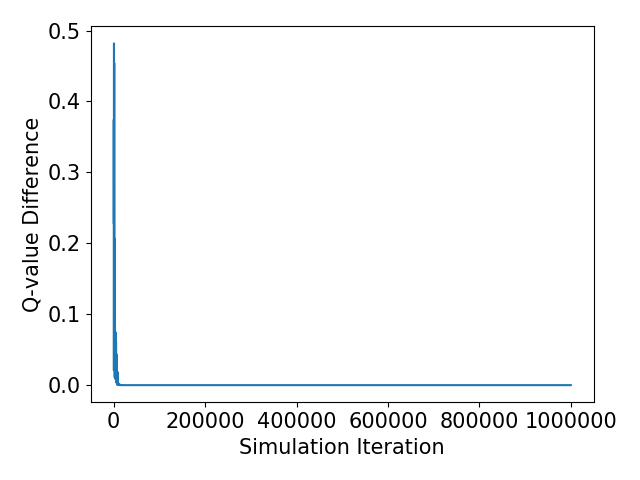
\includegraphics[width=\linewidth]{../figs/Qdifference_29_uncut.png}
      \caption{1 Q table ($\epsilon=1$)}
  \label{fig:friendQ_1Q_1}
  \end{subfigure}
    \begin{subfigure}[b]{0.245\linewidth}
  \centering
  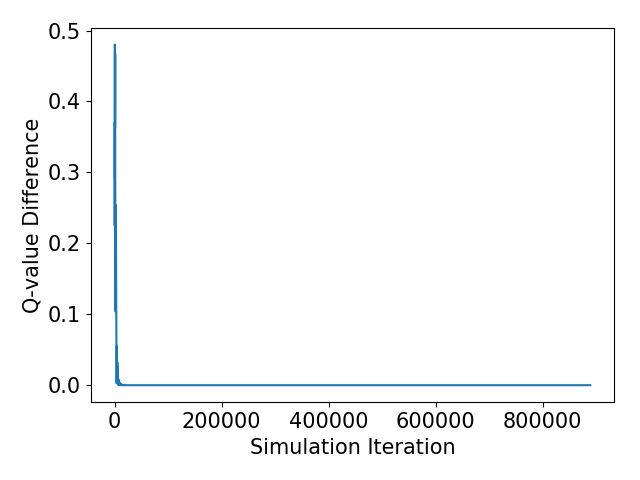
\includegraphics[width=\linewidth]{../figs/Qdifference_28_uncut.png}
      \caption{1 Q table ($\epsilon:1\rightarrow0.001$)}
  \label{fig:friendQ_1Q_0001}
  \end{subfigure}
  \caption{Q-value differences from friend-Q, $\alpha:0.22\rightarrow0.001$. \ul{Here (a) corresponds to Fig 3(c) in Greenwald2003 paper.}\cite{GreenwaldCorrelatedQLearning2003}}
  \label{fig:friendQ}
\end{figure}

%%%%%%%%%%%%%%%%%%% figure here ^

\subsection{Foe-Q} \label{foeQ}
In foe-Q, each agent tries to maximize its own reward and minimize its opponents, and the utility of a particular state $V(s)$ is evaluated to be opposite for the two players. For a zero-sum game like the soccer game discussed in this report, learning two Q tables or a single Q table should both work.\par 
\textbf{Fig} \ref{fig:foeQ_2Q_cut} and \ref{fig:foeQ_2Q_uncut} shows the Q-value differences during training for foe-Q, learning two Q tables, with off-policy $\epsilon$-greedy and $\epsilon=1$ through out learning period (\ul{same as on-policy defined by Greenwald, detailed clarification }see \textbf{Section} \ref{clarification})\cite{GreenwaldCorrelatedQLearning2005}. Different $\alpha$ only changes the scales of Q-value differences, not the result of convergences (data not shown). Learning a single Q table and calculate strategies at maximin equilibrium for both players from the same Q table produces almost identical Q-value difference plot with $\epsilon=1$ (\textbf{Fig} \ref{fig:foeQ_1Q_1}). With $\epsilon:1\rightarrow0.001$, the convergence appears to take slightly more iterations (\textbf{Fig} \ref{fig:foeQ_1Q_0001}), but the result after convergence is unchanged. Foe-Q with all different variations in parameters converged to the same policy for state $s$, as described in the paper\cite{GreenwaldCorrelatedQLearning2003}, $\pi_A(s)\approx[0.5,0,0.5,0,0)]$ and $\pi_B(s)\approx[0.5,0,0.5,0,0)]$. Note that at state $s$, actions N and stick are equivalent for both A and B, sometimes the learning algorithm converges to N, or partially to N, instead of stick, such results should be considered valid.

%%%%%%%%%%%%%%%%%%%figure here v
\begin{figure}[H]
  \centering
  \begin{subfigure}[b]{0.245\linewidth}
  \centering
  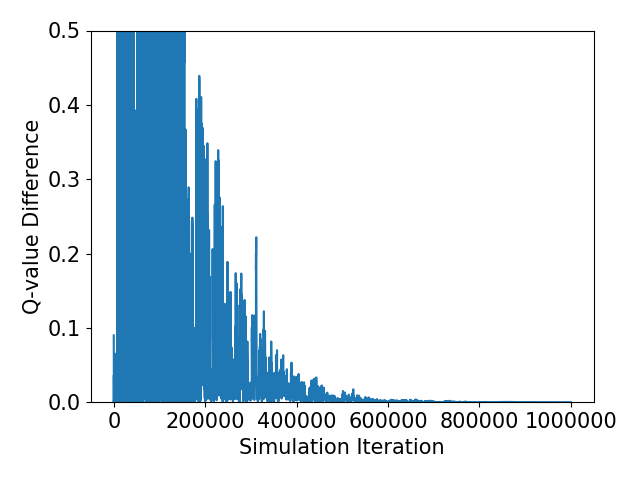
\includegraphics[width=\linewidth]{../figs/foeQ_2Q_09_1_1_1000000_replot.png}
      \caption{$\epsilon=1$, zoomed-in}
  \label{fig:foeQ_2Q_cut}
  \end{subfigure}
  \begin{subfigure}[b]{0.245\linewidth}
  \centering
  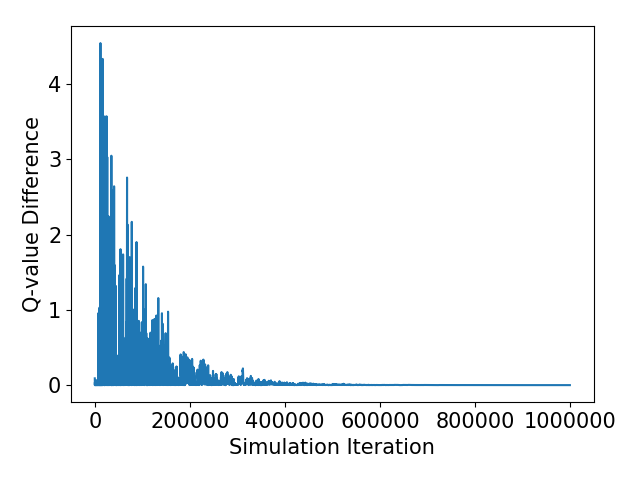
\includegraphics[width=\linewidth]{../figs/foeQ_2Q_09_1_1_1000000.png}
      \caption{$\epsilon=1$, zoomed-out}
  \label{fig:foeQ_2Q_uncut}
  \end{subfigure}
  \begin{subfigure}[b]{0.245\linewidth}
  \centering
  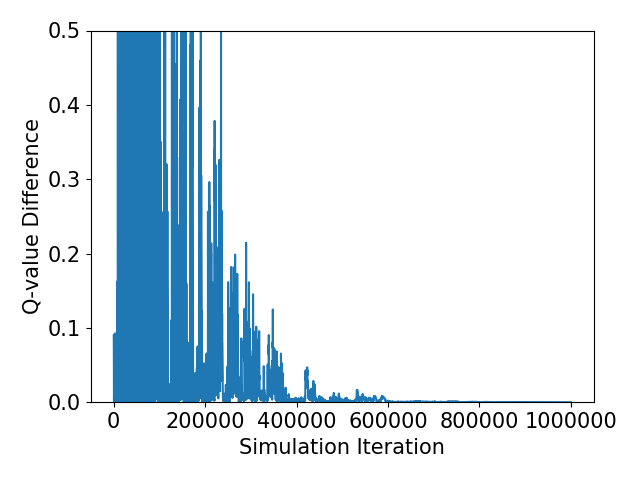
\includegraphics[width=\linewidth]{../figs/Qdifference_11.png}
      \caption{$\epsilon=1$}
  \label{fig:foeQ_1Q_1}
  \end{subfigure}
  \begin{subfigure}[b]{0.245\linewidth}
  \centering
  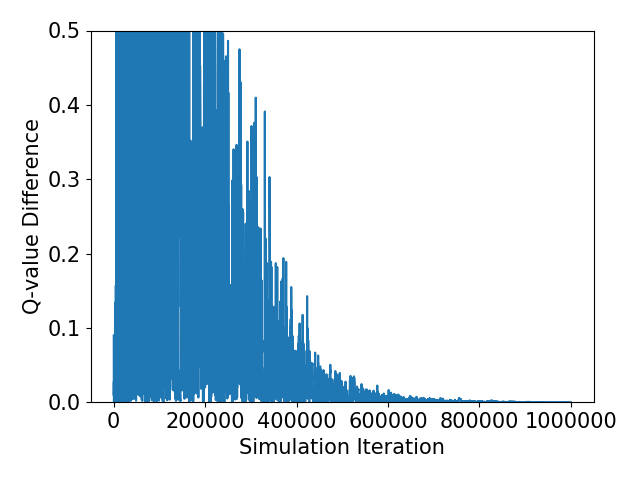
\includegraphics[width=\linewidth]{../figs/Qdifference_7.png}
      \caption{$\epsilon:1\rightarrow0.001$}
  \label{fig:foeQ_1Q_0001}
  \end{subfigure}
  \caption{Q-value differences from foe-Q, by learning 2 Q tables (a and b) and a single Q table (c and d), $\alpha:0.9\rightarrow0.001$. \ul{Here (a) corresponds to Fig 3(b) in Greenwald2003 paper.}\cite{GreenwaldCorrelatedQLearning2003}}
  \label{fig:foeQ}
\end{figure}

%%%%%%%%%%%%%%%%%%% figure here ^

\subsection{CE-Q} \label{ceQ}
CE-Q evaluates the utility at a particulate state $V(s)$ using the mixed strategy of joint actions obtained at a correlated equilibrium. Here the CE-Q learner learns two separate Q tables for A and B, and using Q values from both tables to generate a strategy of joint actions using linear programming. Again, off-policy with both $\epsilon=1$ and $\epsilon:1\rightarrow0.001$ (\ul{or off- and on-policy as Greenwald defined, detailed clarification discussed in }\textbf{Section} \ref{clarification})\cite{GreenwaldCorrelatedQLearning2005} are tested. As shown in \textbf{Fig} \ref{fig:ceQ_1_cut} and \ref{fig:ceQ_1_uncut}, the algorithm converges in the similar manner to foe-Q. By comparing \textbf{Fig} \ref{fig:ceQ_1_cut} and \ref{fig:ceQ_0001_cut}, the algorithm seems to be able to converge faster by always choosing action randomly ($\epsilon=1$), as opposed to $\epsilon$-greedy with $\epsilon:1\rightarrow0.001$. Different $\alpha$ values are also tested, they do not seem make any difference other than changing the scale of Q-value differences, similar to the observations in foe-Q and Q-Learning. CE-Q with all different variations in parameters converged to the same policy for state $s$, as described in the paper\cite{GreenwaldCorrelatedQLearning2003}, $\pi_A(s)\approx[0.5,0,0.5,0,0)]$ and $\pi_B(s)\approx[0.5,0,0.5,0,0)]$. Similar to what was discussed in foe-Q (\textbf{Section} \ref{foeQ}), at state $s$, actions N and stick are equivalent for both A and B, sometimes the learning algorithm converges to N, or partially to N, instead of stick, such results should be considered valid.

%%%%%%%%%%%%%%%%%%%figure here v
\begin{figure}[H]
  \centering
  \begin{subfigure}[b]{0.245\linewidth}
  \centering
  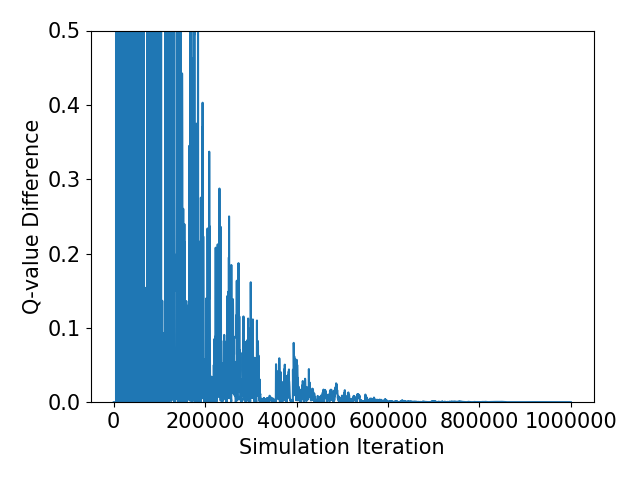
\includegraphics[width=\linewidth]{../figs/ceQ_09_1_1_1000000_replot.png}
      \caption{$\epsilon=1$, zoomed-in}
  \label{fig:ceQ_1_cut}
  \end{subfigure}
  \begin{subfigure}[b]{0.245\linewidth}
  \centering
  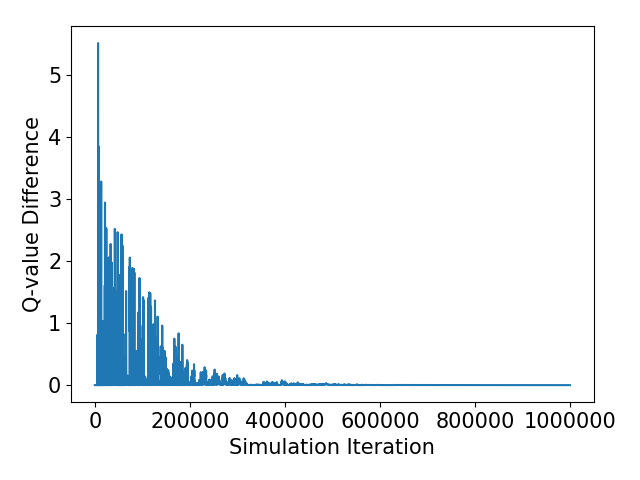
\includegraphics[width=\linewidth]{../figs/ceQ_09_1_1_1000000.png}
      \caption{$\epsilon=1$, zoomed-out}
  \label{fig:ceQ_1_uncut}
  \end{subfigure}
   \begin{subfigure}[b]{0.245\linewidth}
  \centering
  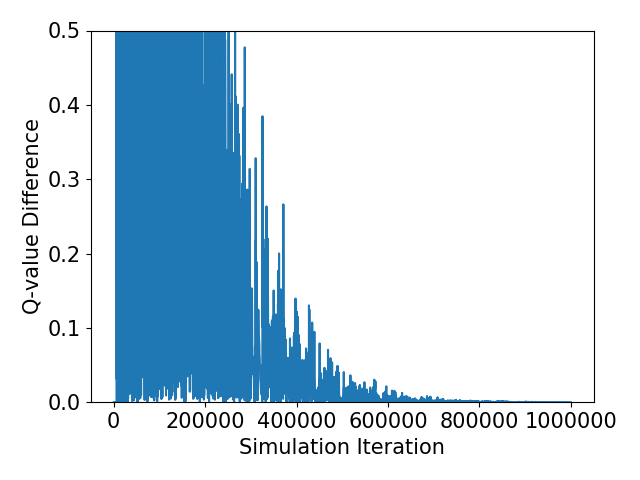
\includegraphics[width=\linewidth]{../figs/Qdifference_9.png}
      \caption{$\epsilon:1\rightarrow0.001$, zoomed-in}
  \label{fig:ceQ_0001_cut}
  \end{subfigure}
  \caption{Q-value differences with CE-Q, $\alpha:0.9\rightarrow0.001$. \ul{Here (a) corresponds to Fig 3(a) in Greenwald2003 paper.}\cite{GreenwaldCorrelatedQLearning2003}}
  \label{fig:ceQ}
\end{figure}

%%%%%%%%%%%%%%%%%%% figure here ^


%%%%%%%%%%%%%%%%%%%%%%figure here v
%%%%%%%%%%%%%%%%%%%%%%figure here ^


%\section{Appendix} \label{appendix}
%Code used to run experiments described in this report is hosted here: \burl{https://github.gatech.edu/rchen350/cs7642summer2018p3}. 

\bibliographystyle{unsrt}
\bibliography{ref}

\end{document}
















